\documentclass{report}
\usepackage{graphicx}
\usepackage{amsmath}
\usepackage{amssymb}
\usepackage{amsthm}
\usepackage{algorithm}
\usepackage{algpseudocode}
\usepackage{hyperref}
\usepackage{enumitem}
\usepackage{multirow}

\title{CS728: Assignment 1}
\author{Jay Mehta: 22B1281\\
        Kshitij Vaidya: 22B1829\\
        Tanay Bhat: 22B3303}
\date{\today}  

\begin{document}

\maketitle

\tableofcontents

\chapter{Task 1}

The following table shows the final parameters used for the Glove training:
\begin{table}[h]
    \centering
    \begin{tabular}{cc}
        \hline
        Hyperparameter & Value \\
        \hline
        Window Size ($w$) & 10 \\
        Learning Rate ($\eta$) & 0.05 \\
        Epochs & 25 \\
        $x_{\max}$ & 100 \\
        $\alpha$ & 0.75 \\
        \hline
    \end{tabular}
    \caption{Selected GloVe hyperparameters}
\end{table}

\noindent Nearest Neighbours for this task have been mentioned with results of Task 2.

\begin{figure}[!htbp]
    \centering
    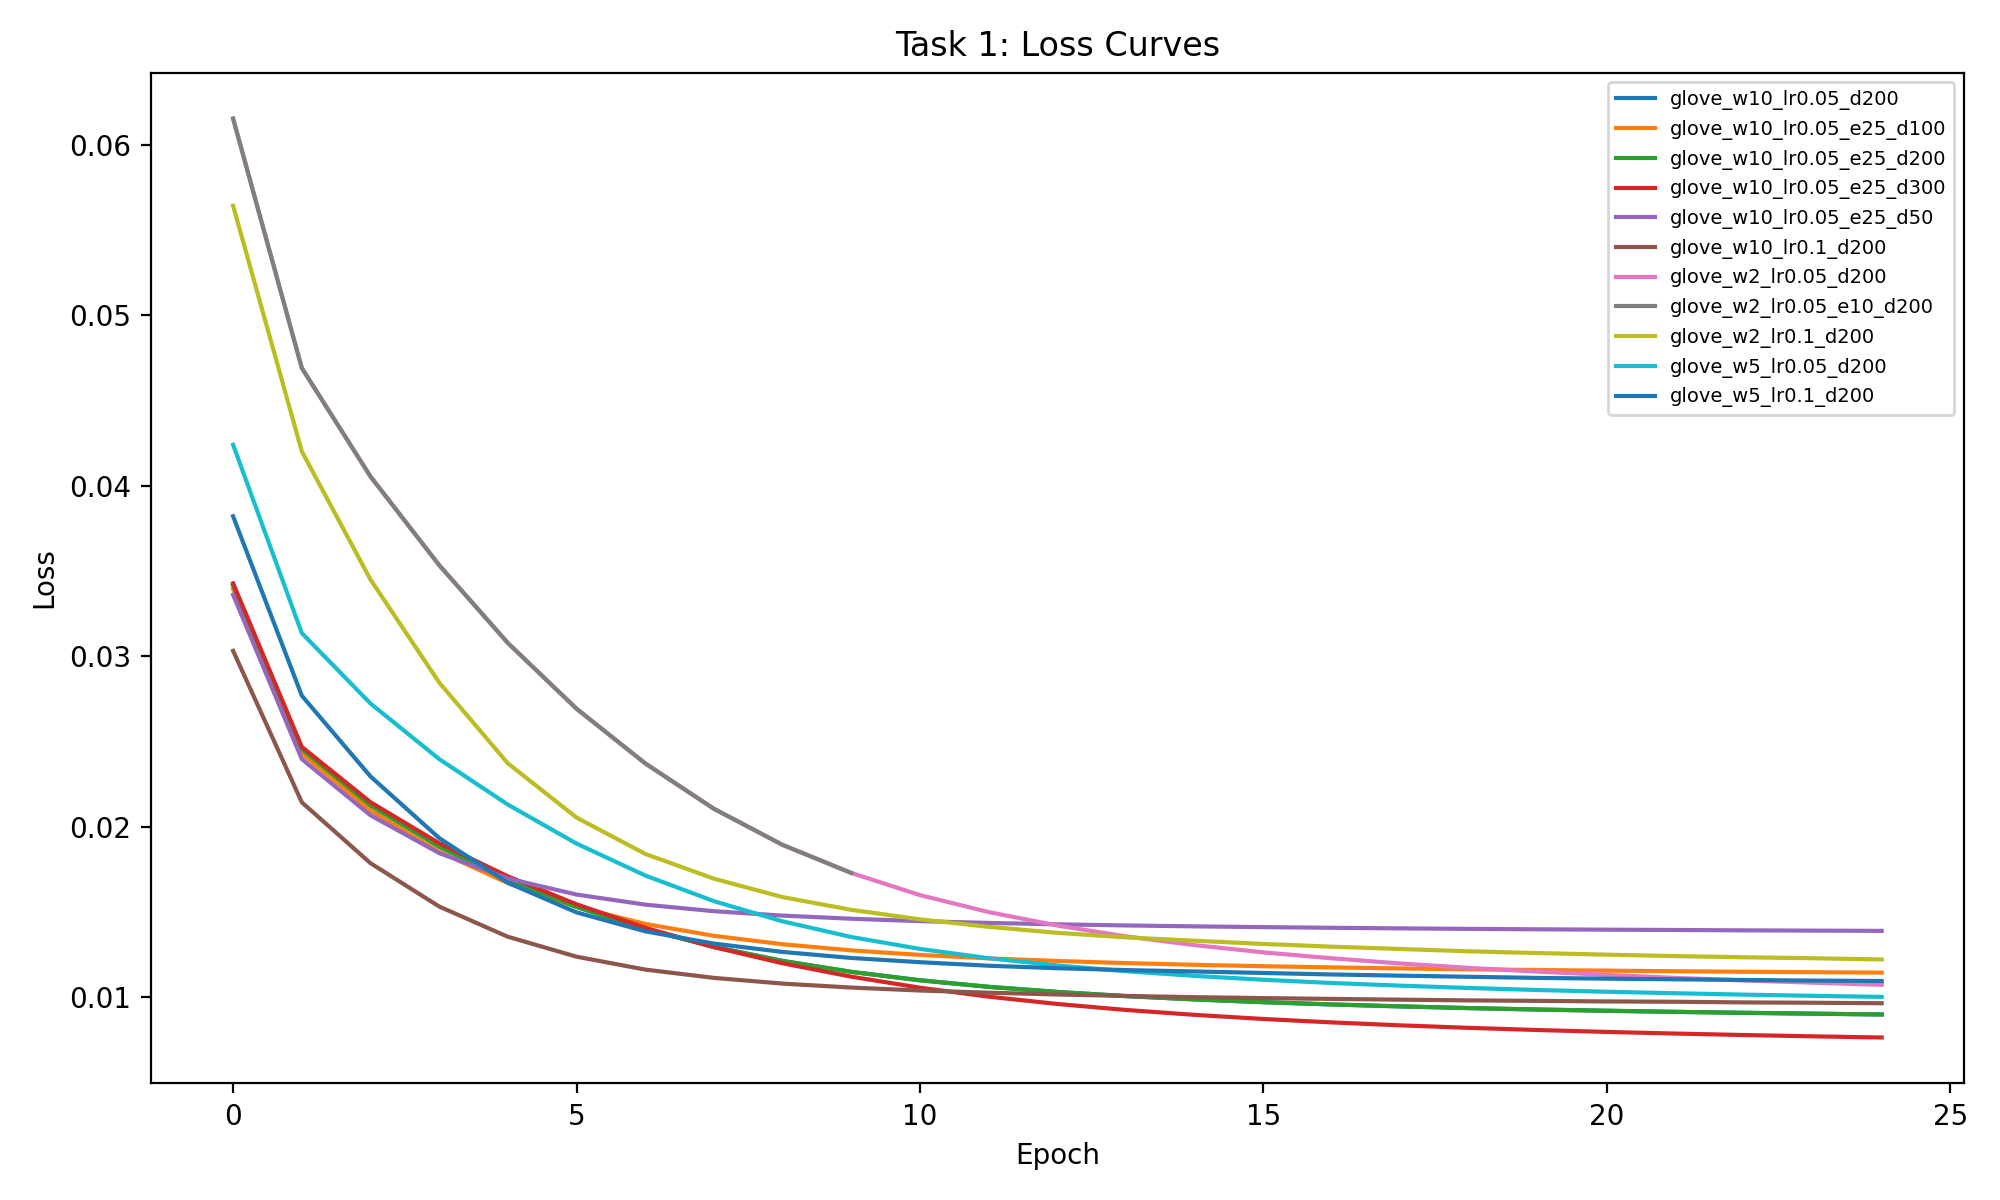
\includegraphics[width=0.8\textwidth]{plots/task1_loss_curves.png}
    \caption{Loss curves for different embedding dimensions}
\end{figure}

\newpage
\begin{figure}[!htbp]
    \centering
    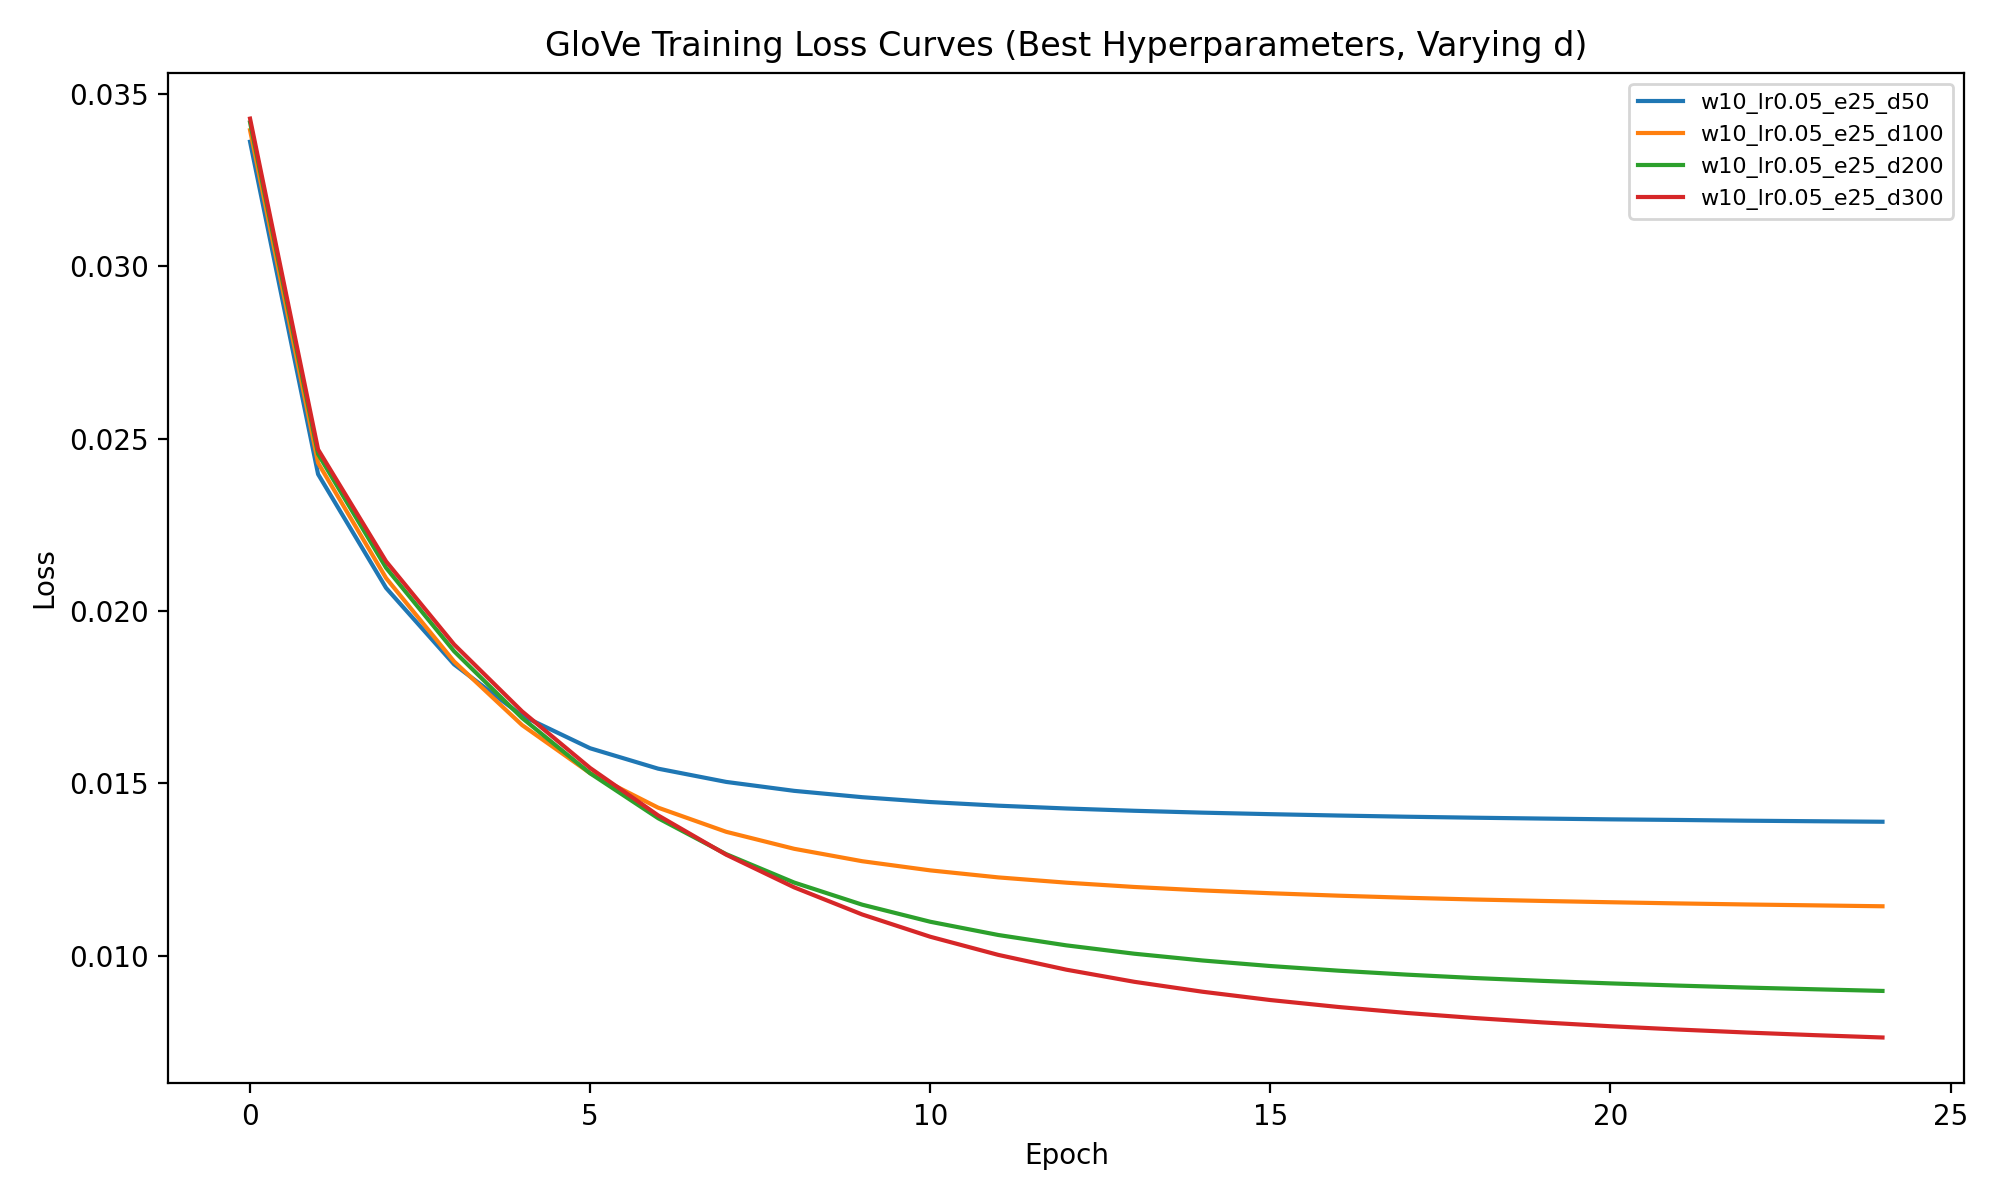
\includegraphics[width=0.8\textwidth]{plots/task1_loss_curves_by_dimension.png}
    \caption{Loss curves for best hyperparameters across embedding dimensions}
\end{figure}

\begin{figure}[!htbp]
    \centering
    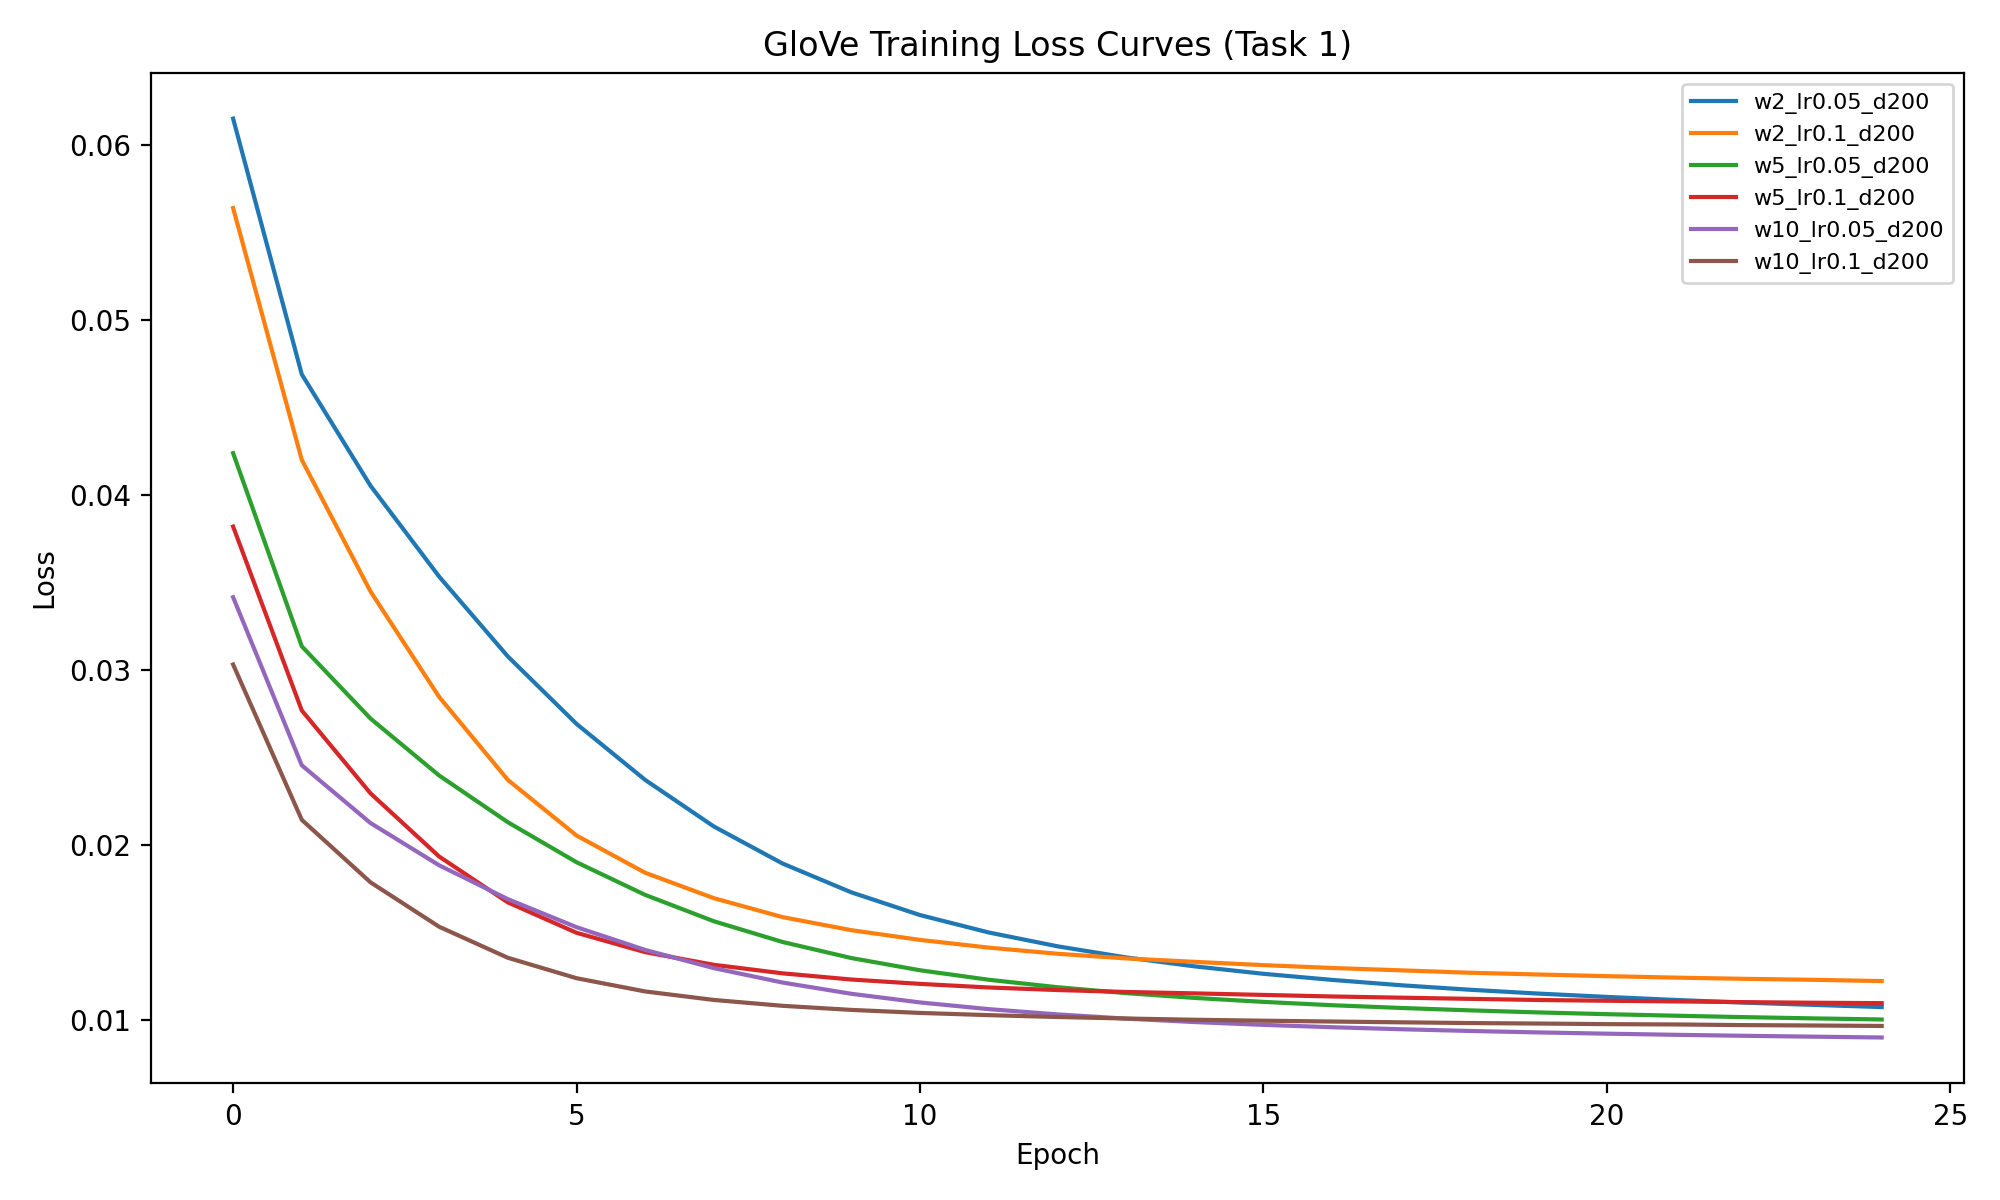
\includegraphics[width=0.8\textwidth]{plots/task1_loss_curves_d200.png}
    \caption{Loss curves for embedding dimension 200}
\end{figure}

\newpage
\begin{figure}[!htbp]
    \centering
    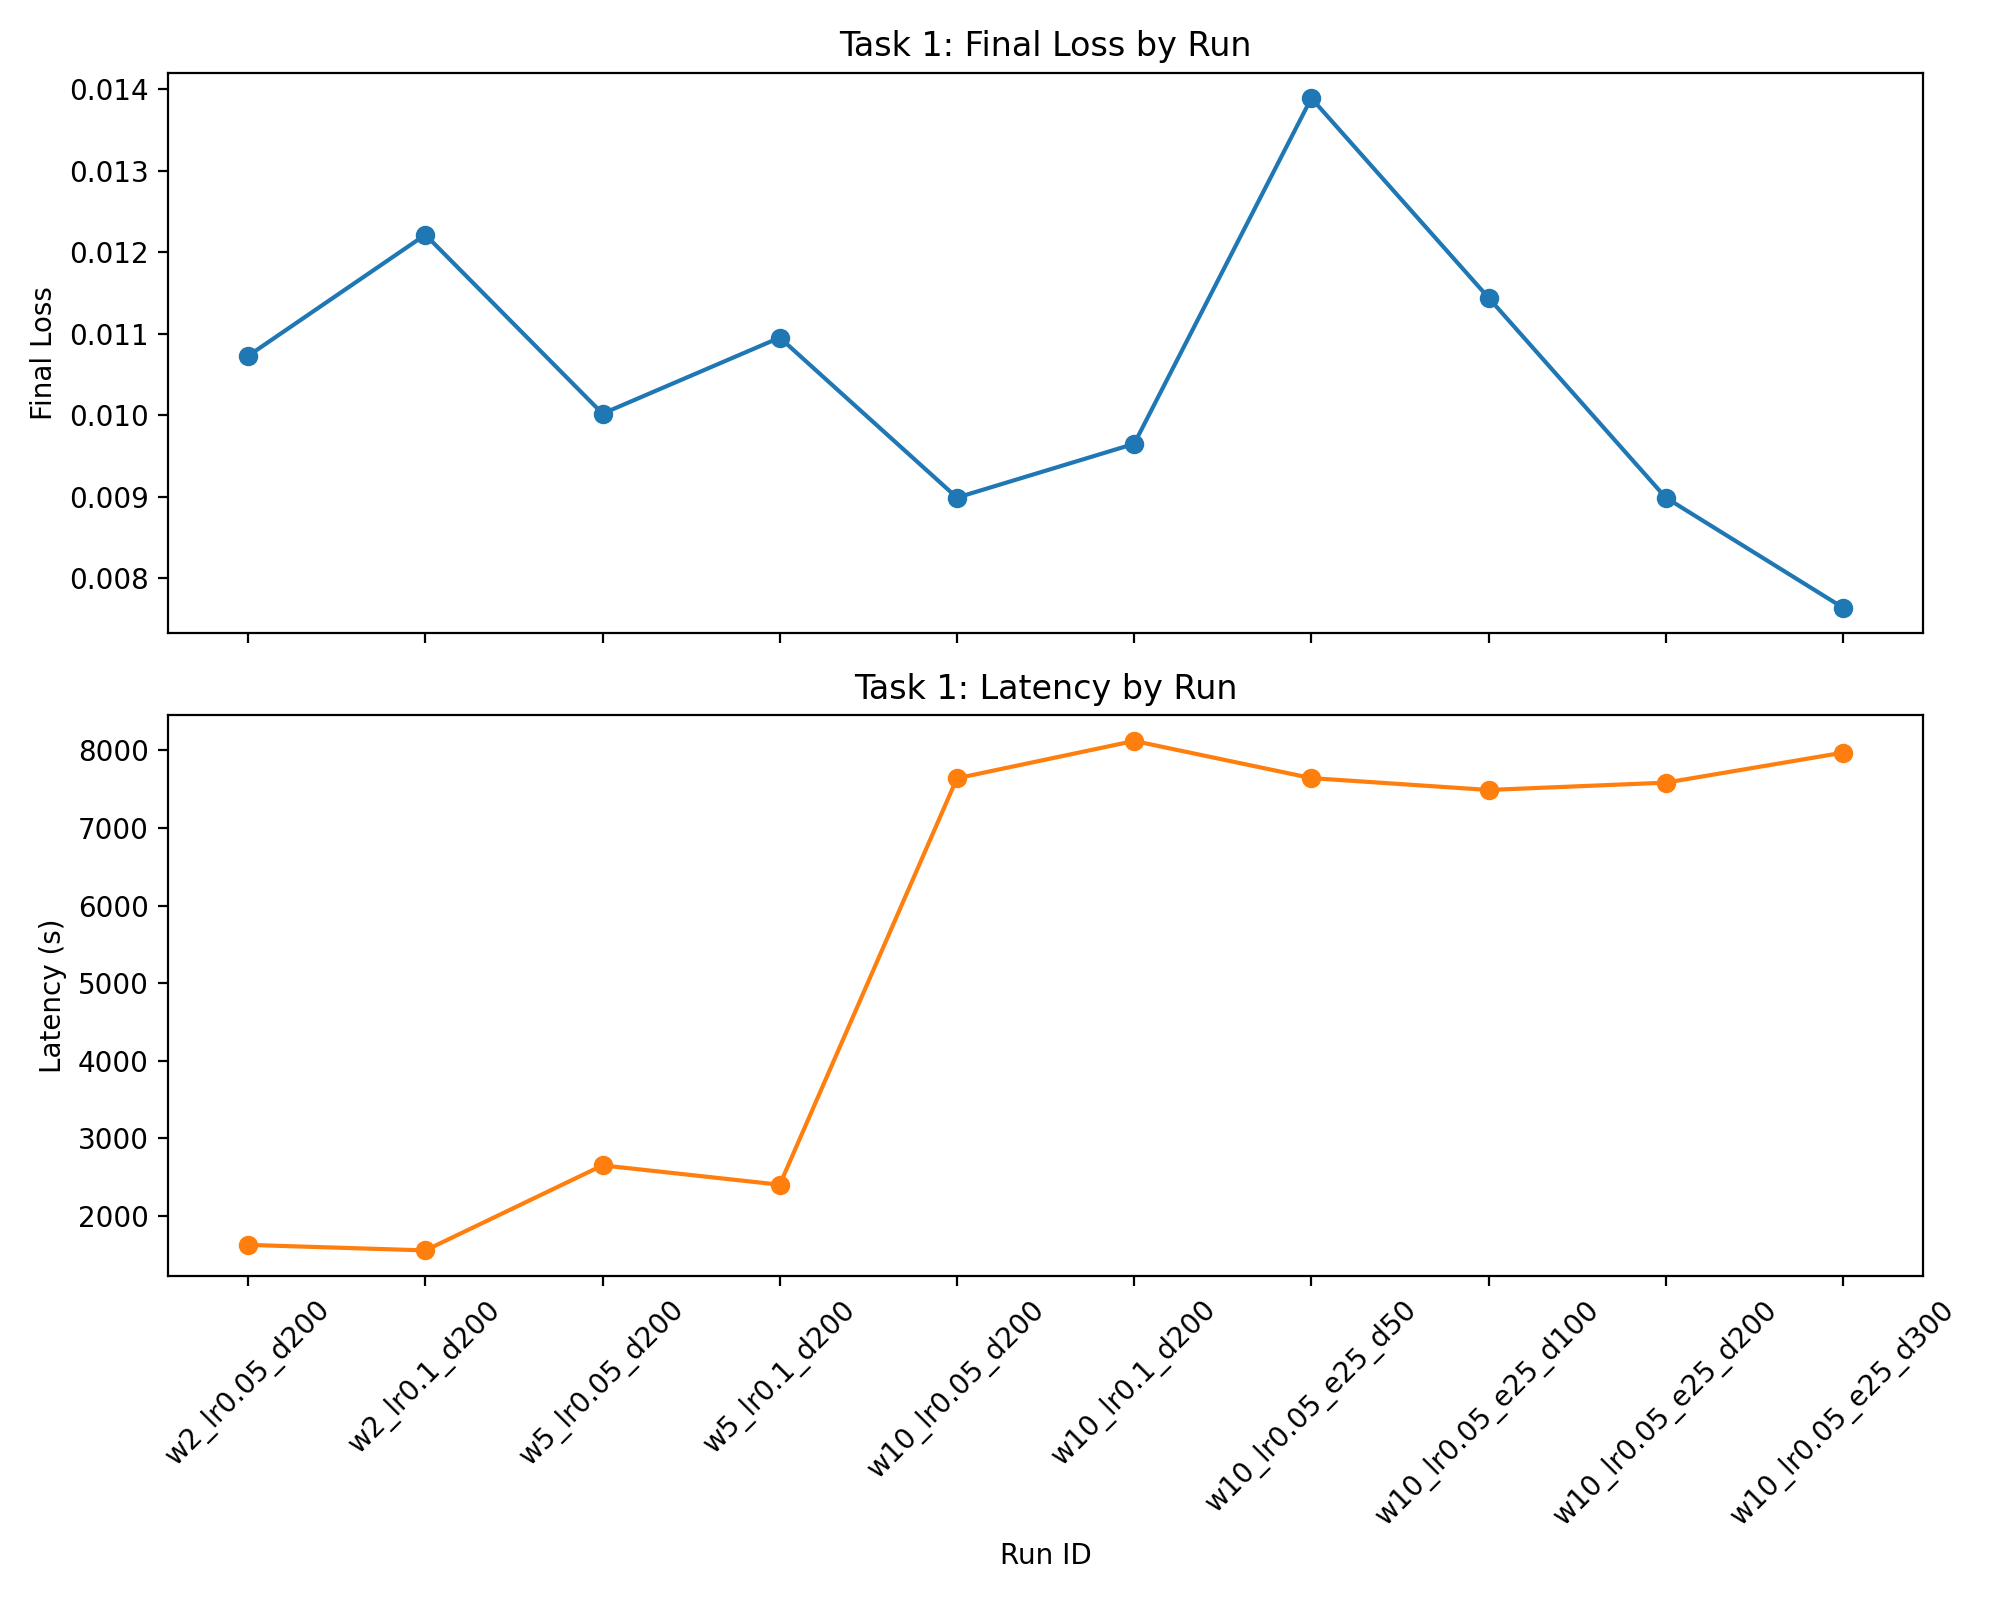
\includegraphics[width=0.8\textwidth]{plots/task1_loss_latency.png}
    \caption{Final loss and Latency for different hyperparameters}
\end{figure}


\chapter{Task 2}

\begin{table}[h]
\centering
\begin{tabular}{ccc}
\hline
Model & Word & Top-5 Neighbours \\
\hline
\multirow{3}{*}{GloVe (d=200)} & data & showed, statistics, tracking, according, information \\
 & cities & towns, counties, across, areas, twin \\
 & temperature & temperatures, maximum, levels, rainfall, room \\
\hline
\multirow{3}{*}{SVD (d=50)} & data & consumers, risk, tracking, technology, exposure \\
 & cities & urban, influx, airports, communities, places \\
 & temperature & heating, severe, fog, checking, causes \\
\hline
\multirow{3}{*}{SVD (d=100)} & data & automated, rapid, tool, specific, tracking \\
 & cities & urban, transit, places, tourism, suburbs \\
 & temperature & skin, heating, pump, cold, dry \\
\hline
\multirow{3}{*}{SVD (d=200)} & data & infrastructure, authentication, formulated, users, est \\
 & cities & urban, mayor, city, transit, vast \\
 & temperature & cold, slow, evaporate, brush, water \\
\hline
\multirow{3}{*}{SVD (d=300)} & data & mainframe, users, collected, infrastructure, breach \\
 & cities & urban, city, mayor, vast, places \\
 & temperature & cold, temperatures, evaporate, surface, fluids \\
\hline
\end{tabular}
\caption{Top-5 nearest neighbours for selected words in GloVe and SVD models}
\end{table}

\chapter{Task 3}

The final parameters used for the CRF model were:

\begin{table}[h]
    \centering
    \begin{tabular}{cc}
        \hline
        Parameter & Value \\
        \hline
        include\_lexical & True \\
        include\_shape & True \\
        include\_subword & True \\
        window\_size & 2 \\
        \hline
    \end{tabular}
    \caption{CRF model parameters}
\end{table}

\begin{table}[h]
\centering
\small
\begin{tabular}{ll}
\hline
\textbf{Category} & \textbf{Features} \\
\hline

Bias & bias \\

\hline
Lexical (Current Token) &
word.lower, pos, chunk, pos[:2] \\

\hline
Lexical (Context $\pm 1$) &
-1:word.lower, -1:pos, -1:chunk \\
&
+1:word.lower, +1:pos, +1:chunk \\

\hline
Lexical (Context $\pm 2$) &
-2:word.lower, -2:pos, -2:chunk \\
&
+2:word.lower, +2:pos, +2:chunk \\

\hline
Shape (Current Token) &
word.isupper, word.istitle, word.isdigit, \\
&
word.shape, word.has\_digit, \\
&
word.has\_hyphen, word.has\_period \\

\hline
Shape (Context $\pm 1$) &
-1:word.isupper, -1:word.istitle, -1:word.isdigit, -1:word.shape \\
&
+1:word.isupper, +1:word.istitle, +1:word.isdigit, +1:word.shape \\

\hline
Shape (Context $\pm 2$) &
-2:word.isupper, -2:word.istitle, -2:word.isdigit, -2:word.shape \\
&
+2:word.isupper, +2:word.istitle, +2:word.isdigit, +2:word.shape \\

\hline
Subword &
pref2, pref3, pref4, suf2, suf3, suf4 \\

\hline
Sentence Boundary &
BOS1, EOS1, BOS2, EOS2 \\

\hline
\end{tabular}
\caption{Complete feature set used with window size = 2}
\end{table}

The table below lists the most important features learned:

\begin{table}[h]
\centering
\small
\begin{tabular}{lll}
\hline
\textbf{Type} & \textbf{Feature} & \textbf{Weight} \\
\hline

State & word.shape:x $\rightarrow$ O & 5.9832 \\
State & word.has\_digit $\rightarrow$ O & 5.2317 \\
State & word.shape:x\_x $\rightarrow$ O & 4.8745 \\
State & +2:word.lower=yellow $\rightarrow$ B-LOC & 4.1123 \\
State & -1:word.lower=v $\rightarrow$ B-ORG & 3.9864 \\
State & word.shape:Xx $\rightarrow$ B-PER & 3.7421 \\
State & pref3=mc $\rightarrow$ B-PER & 3.6158 \\
State & suf3=son $\rightarrow$ I-PER & 3.5084 \\
State & word.isupper=True $\rightarrow$ B-ORG & 3.4219 \\
State & word.istitle=True $\rightarrow$ B-PER & 3.3376 \\

\hline
Transition & B-PER $\rightarrow$ I-PER & 6.4821 \\
Transition & B-LOC $\rightarrow$ I-LOC & 6.1734 \\
Transition & B-ORG $\rightarrow$ I-ORG & 5.9648 \\
Transition & I-LOC $\rightarrow$ I-LOC & 5.4127 \\
Transition & O $\rightarrow$ I-PER & -6.2354 \\
Transition & O $\rightarrow$ I-ORG & -6.0112 \\
Transition & O $\rightarrow$ I-LOC & -5.8846 \\
Transition & I-PER $\rightarrow$ I-PER & 4.9731 \\
Transition & I-ORG $\rightarrow$ I-ORG & 4.8265 \\
Transition & B-MISC $\rightarrow$ I-MISC & 4.7029 \\

\hline
\end{tabular}
\caption{Top CRF features ranked by absolute weight magnitude.}
\end{table}



\chapter{Task 4}

We used a simple MLP architecture with a single hidden layer with 128 neurons followed by a ReLU and a dropout layer with a dropout rate of 0.2. The final output layer has 9 neurons corresponding to the 9 classes in the dataset. For OOV words we use the mean of the embeddings of the words in the training set as the embedding for the OOV word as it acts like a neutral embedding and does not bias the model towards any particular class. We trained the model for 10 epochs with a batch size of 1024 and a learning rate of 0.001 using the Adam optimizer. The tables below show the results of our model on the test set. 

\begin{table}[h]
\centering
\begin{tabular}{cccc}
\hline
Dimension & Accuracy & Weighted F1 & Macro F1 \\
\hline
50  & 0.8309 & 0.7619 & 0.2179 \\
100 & 0.8314 & 0.7643 & 0.2198 \\
200 & 0.8314 & 0.7653 & 0.2224 \\
300 & 0.8319 & 0.7658 & 0.2241 \\
\hline
\end{tabular}
\caption{Test performance of GloVe-MLP across embedding dimensions}
\end{table}

\begin{table}[h]
\centering
\begin{tabular}{cccc}
\hline
Dimension & Accuracy & Weighted F1 & Macro F1 \\
\hline
50  & 0.8274 & 0.7523 & 0.2043 \\
100 & 0.8301 & 0.7589 & 0.2091 \\
200 & 0.8309 & 0.7609 & 0.2126 \\
300 & 0.8305 & 0.7607 & 0.2118 \\
\hline
\end{tabular}
\caption{Test performance of SVD-MLP across embedding dimensions}
\end{table}

From this we see that the best performance is achieved with the GloVe embeddings with a dimension of 300 and the SVD embeddings with a dimension of 200. This is worse than the CRF model which achieved macro F1 of 0.7983 and weighted F1 of 0.8342. This is because CRF model uses a window and hence has contextual information whereas and MLP trains on just the current wrord and does not have any context.

\begin{figure}[!htbp]
    \centering
    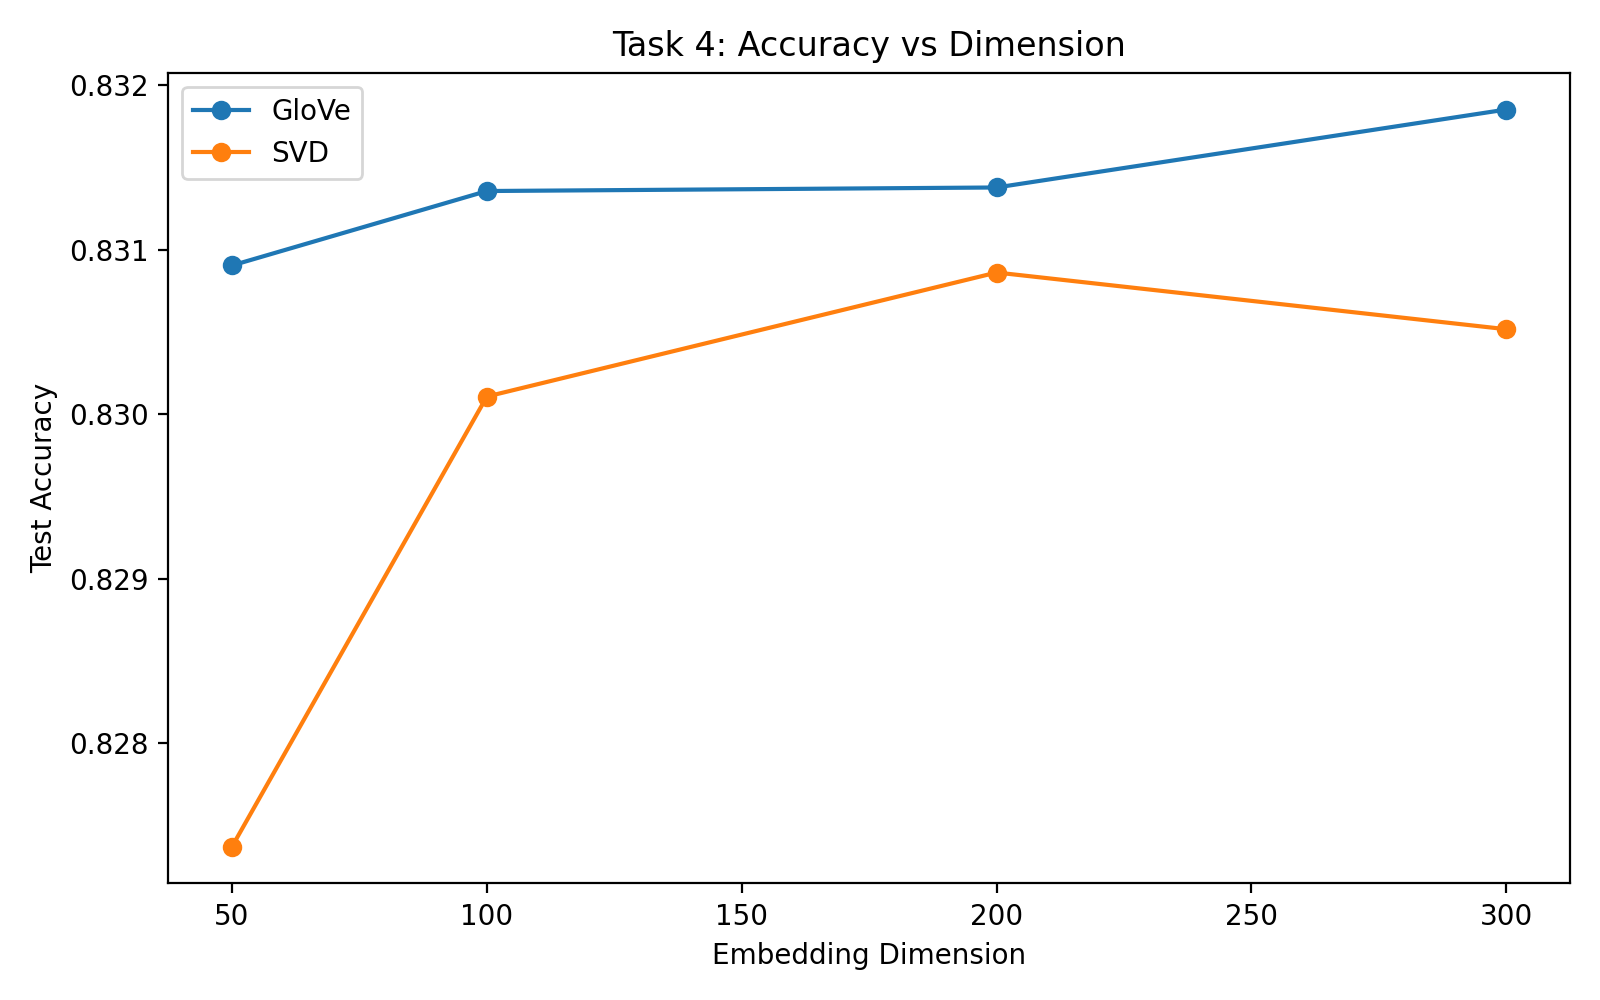
\includegraphics[width=0.8\textwidth]{plots/task4_accuracy.png}
    \caption{Test accuracy across embedding dimensions}
\end{figure}

\begin{figure}[!htbp]
    \centering
    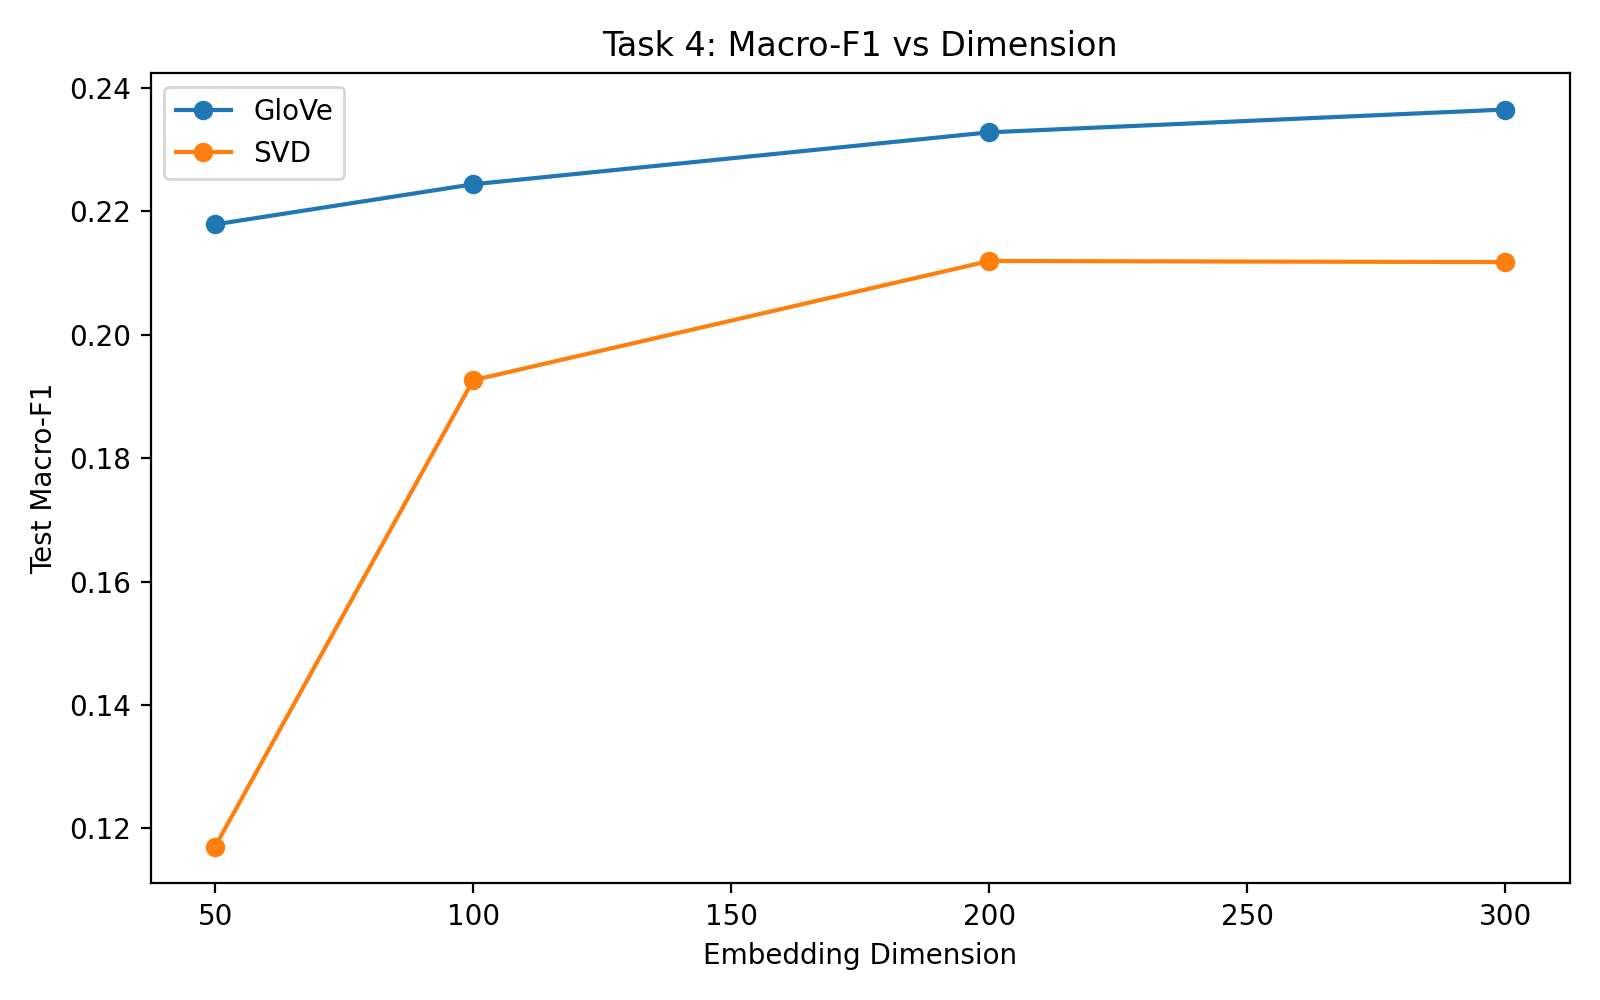
\includegraphics[width=0.8\textwidth]{plots/task4_macro_f1.png}
    \caption{Test F1 score across embedding dimensions}
\end{figure}

\chapter{Task 5}

\begin{table}[h]
\centering
\begin{tabular}{ccc}
\hline
Model & Word & Top-5 Neighbours \\
\hline
\multirow{5}{*}{Raw SVD (d=200)} & data & infrastructure, authentication, formulated, users, est \\
 & temperature & cold, slow, evaporate, brush, water \\
 & cities & urban, mayor, city, transit, vast \\
 & apple & Not in vocabulary \\
 & fast & enough, hard, keep, make, stopping \\
\hline
\multirow{5}{*}{TFIDF SVD (d=200)} & data & formulated, infrastructures, reads, est, mentioning \\
 & temperature & cold, evaporate, temperatures, climatologist, gases \\
 & cities & urban, inexorable, mayor, city, vast \\
 & apple & Not in vocabulary \\
 & fast & enough, hard, quick, make, up \\
\hline
\end{tabular}
\caption{Comparison of Top-5 nearest neighbours for selected words in raw-SVD and TFIDF-SVD models}
\end{table}

The MLP architecture was the same as the one used in task 4. The tables below show the results of our model on the test set.

\begin{table}[h]
\centering
\begin{tabular}{lccc}
\hline
Embedding & Accuracy & Weighted F1 & Macro F1 \\
\hline
SVD (Raw, d=200)   & 0.8287 & 0.7627 & 0.2163 \\
SVD (TF-IDF, d=200) & 0.8297 & 0.7625 & 0.2179 \\
\hline
\end{tabular}
\caption{Test performance comparison between Raw SVD and TF-IDF SVD embeddings (d=200)}
\end{table}

We see that the TF-IDF embeddings perform marginally better than SVD. 

\end{document}

